\documentclass[
    11pt,
    spanish,
    a4paper
]{article}
\usepackage[utf8]{inputenc}
\usepackage[spanish]{babel}
\usepackage{authoraftertitle}
\usepackage{booktabs}
\usepackage{caption}
\usepackage{float}
\usepackage{graphicx}
\usepackage{listings}
\usepackage{verbatim}

\def\doctype{INFORME DE INVESTIGACIÓN}
\title{Softwares de simulación para Tecnología electrónica y otras cátedras de ingeniería}
\author{Gonzalo Nahuel Vaca}

\begin{document}

\makeatletter
\begin{titlepage}
	\begin{center}
		\vspace*{1cm}

		\Huge
		\textbf{\doctype}
		\vspace{0.5cm}

		\LARGE
		\@title
		\vspace{0.5cm}

		\textbf{Compatibilidad electromagnética}

		\vspace{1.5cm}

		\textbf{\@author}

		\vspace{1.5cm}

		
\includegraphics[width=0.4\textwidth]{img/logoUNLaM.png}

		\vfill
		Universidad Nacional de la Matanza\\
		Argentina\\
		\today
	\end{center}
\end{titlepage}
\makeatother
\newpage

\section*{Resumen}

Este informe es una memoria breve del trabajo realizado durante el año 2022.
En el marco de la investigación se evaluaron distintos programas para el análisis de compatibilidad electromagnética.

\section{Compatibilidad electromagnética}

Esta sección es una introducción a la temática que abordan los programas evaluados; su naturaliza e importancia.

% temática

El diseño de circuitos electrónicos que manejan señales de alta frecuencia se someten a efectos no deseados.
Esto se debe a que las trazas del impreso son fuentes de radiación electromagnética.
Luego, se inducen corrientes en las pistas cercanas que pueden alterar o destruir parte del sistema.
Además, las ecuaciones que rigen el comportamiento de la radiación en el circuito impreso son de gran complejidad.

Es posible construir guías de onda en un circuito impreso, como así también filtros y blindajes.
También es posible dibujar adaptadores de impedancia para conectar una antena.
En la figura \ref{fig:pcb} se puede observar un ejemplo de un circuito que implementa estos componentes como parte de sus trazas.

\begin{figure}[htbp]
	\centering
	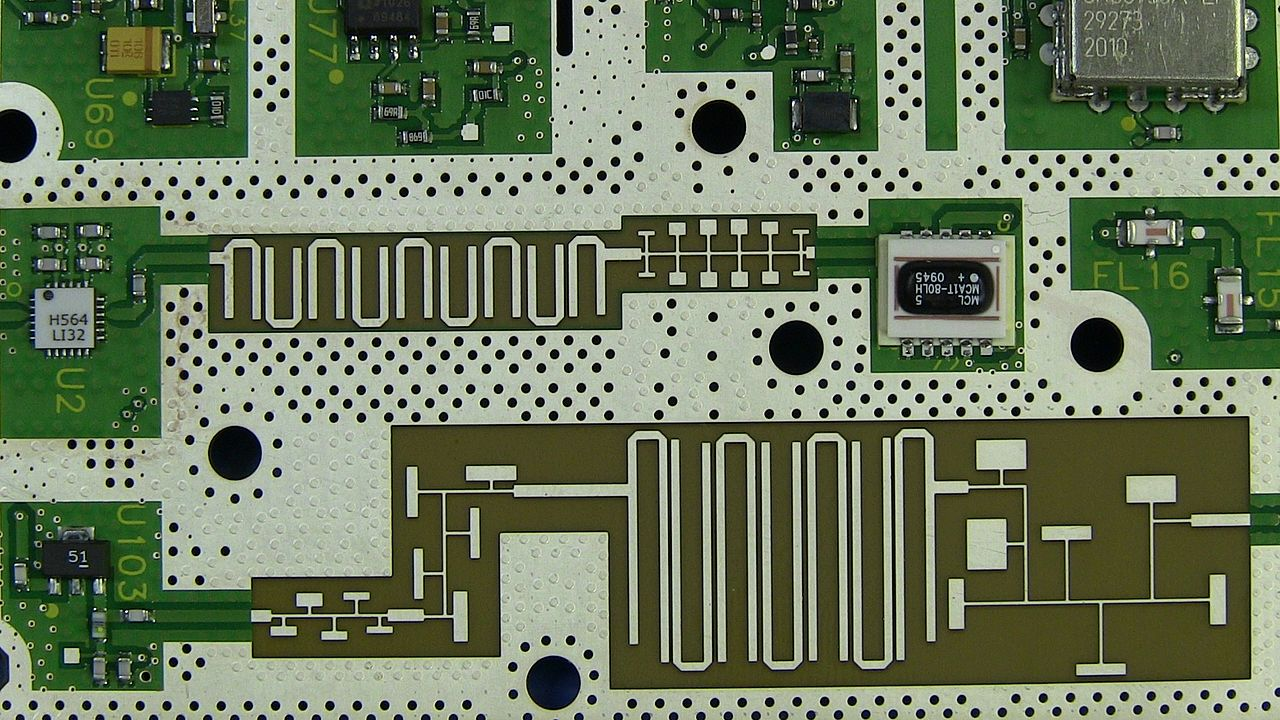
\includegraphics[width=0.8\textwidth]{img/pcb.jpg}
	\caption{Guías de ondas, filtros, adaptadores y blindajes impresos.}
	\label{fig:pcb}
\end{figure}

Los componentes modernos tienen un alto grado de integración y a menudo manejan señales de alta frecuencia.
Los encapsulados tienen un gran número de terminales que en algunos casos obligan a crear un circuito impreso donde las pistas de alta frecuencia se encuentran en proximidad.
En la figura \ref{fig:fpga} se puede ver una \emph{field-programable gate array} (FPGA) y se puede apreciar la cercanía de sus terminales.
Además, este tipo de componente se suele utilizar en una cadena de procesamiento de datos de alta frecuencia.
Finalmente, se pone de manifiesto la necesidad de utilizar una herramienta informática para asistir en el cálculo y simulación de la física involucrada.

\begin{figure}[htbp]
	\centering
	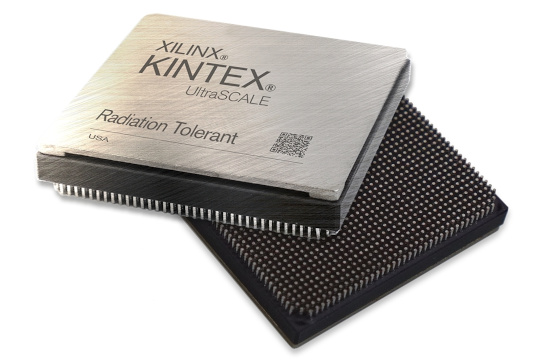
\includegraphics[width=0.6\textwidth]{img/fpga.jpg}
	\caption{Componente de alto grado de integración.}
	\label{fig:fpga}
\end{figure}

Los programas evaluados utilizan el método de elementos finitos (FEM). El cuál permite resolver numéricamente ecuaciones diferenciales que de la geometría del circuito y de las señales que lo estimulan.
Esta estrategia se utiliza en distintos tipos de simulación como: análisis estructural, transferencia de calor, flujo de fluidos, transporte de masa y potencial electromagnético.

El FEM es un método numérico general para resolver ecuaciones diferenciales parciales en dos o tres variables espaciales (es decir, algunos problemas de valores en la frontera).
Para resolver un problema, el FEM subdivide un sistema grande en partes más pequeñas y simples que se denominan elementos finitos.
Esto se logra mediante una discretización espacial particular en las dimensiones del espacio, que se implementa mediante la construcción de una malla del objeto: el dominio numérico para la solución, que tiene un número finito de puntos.
La formulación del método de elementos finitos de un problema de valores en la frontera finalmente da como resultado un sistema de ecuaciones algebraicas.
El método aproxima la función desconocida sobre el dominio.
Las ecuaciones simples que modelan estos elementos finitos se ensamblan luego en un sistema de ecuaciones más grande que modela todo el problema.
Luego, el FEM aproxima una solución minimizando una función de error asociada a través del cálculo de variaciones.

En la figura \ref{fig:simulacion_ejemplo} se puede observar el resultado de una simulación por el método FEM.

\begin{figure}[htbp]
	\centering
	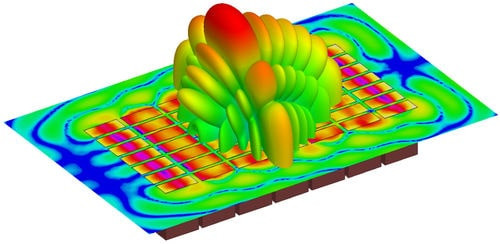
\includegraphics[width=0.8\textwidth]{img/simulacion_1_01.jpg}
	\caption{Simulación de un circuito impreso.}
	\label{fig:simulacion_ejemplo}
\end{figure}

\newpage

\section{OpenEMS}

En esta sección se encuentran los detalles de la evaluación del programa OpenEMS.

\subsection{Introducción}

El programa OpenEMS fue escrito en el lenguaje C++ y utiliza el método de las diferencias finitas en el dominio temporal (FDTD) para resolver simulaciones electromagnéticas.

El programa fue pensado originalmente para realizar simulaciones de equipos médicos de resonancia magnética (MRI).
Sin embargo, se desarrolló un analizador léxico que permite transformar el formato \emph{Hyperlynx} que utiliza KiCad al esquema de geometría de OpenEMS.

El modelo geométrico de OpenEMS es \emph{CSXCAD} y es una biblioteca propia del programa.
Además, permite su visualización y trabajo en coordenadas cartesianas y cilíndricas.
Finalmente, provee una interfaz para Matlab/Octave y Python.

Las características más relevantes son:

\begin{itemize}
	\item Diseño y simulación en coordenadas cartesianas.
	\item Diseño y simulación en coordenadas cilíndricas.
	\item Soporta modelos \emph{voxel} para simulaciones MRI.
	\item Multi-hilos y SIMD.
	\item Intefaz Matlab/Octave.
	\item Definición de materiales en el espacio.
	\item Definición de excitaciones en el espacio.
	\item Generación de archivos en formato \emph{vtk} y \emph{hdf5}
	\item Materiales dispersivos(Drude/Lorentz/Debye)
	\item Rutinas de post-procesamiento configurables (Matlab/Octave).
	\item Sub-espacios de simulación para optimizar densidades de cálculo.
	\item Simulaciones remotas por medio de \emph{ssh}.
	\item Es libre y gratuito.
\end{itemize}

Se creó un entorno de trabajo en Ubuntu 2020 y en contenedores de \emph{docker} para las versiones de Ubuntu 2018 y 2016.
Además se estudió como utilizarlo con Octave y se obtuvieron los siguientes resultados:

\begin{itemize}
	\item El analizador léxico se encuentra abandonado y no es posible hacerlo funcionar
	\item KiCad 6 cambió su formato \emph{Hyperlynx} y el analizador léxico es por lo tanto obsoleto.
	\item Las geometrías de los circuitos impresos se deben construir a mano.
	\item Los errores de geometría no son útiles para depurar los datos ingresados.
\end{itemize}

Dado el estado actual de este programa se hace imposible utilizarlo como herramienta de las cátedras si antes no se repara y actualiza el analizador léxico.

En la figura \ref{fig:openems} se puede observar una simulación realizada en OpenEMS.

\begin{figure}[htbp]
	\centering
	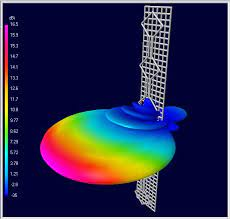
\includegraphics[width=0.7\textwidth]{img/openems.jpeg}
	\caption{Simulación una antena en OpenEMS.}
	\label{fig:openems}
\end{figure}

\subsection{Instalación}
\label{sub:oinstalacion}

La instalación del programa no es trivial y a continuación se detallan los pasos a seguir para tener el programa en funcionamiento.
Esto tiene la finalidad de demostrar la dificultad que enfrentaría el cuerpo de estudiantes y docentes.

A continuación se detallan los pasos a seguir:

\begin{enumerate}
  \item Satisfacer las dependencias del programa, a continuación se muestran los
    comandos para el sistema Ubuntu 22.04 LTS:
    \begin{itemize}
      \item Dependencias mínimas obligatorias:\\
        \texttt{sudo apt-get install\\
        build-essential cmake git libhdf5-dev libvtk7-dev\\
        libboost-all-dev libcgal-dev libtinyxml-dev\\
        qtbase5-dev libvtk7-qt-dev}
      \item GNU Octave (equivalente GNU de Matlab, opcional):\\
        \texttt{sudo apt-get install octave liboctave-dev}
      \item Interfaz Python (opcional):\\
        \texttt{sudo pip3 install matplotlib cython h5py}
    \end{itemize}
  \item Clonar e instalar
    \begin{itemize}
      \item Clonar el repositorio y sus submódulos:\\
        \texttt{git clone --recursive\\
          https://github.com/thliebig/openEMS-Project.git}
      \item Dentro del repositorio ejecutar:
        \begin{verbatim}
./update_openEMS.sh ~/opt/openEMS --python
        \end{verbatim}
    \end{itemize}
\end{enumerate}

\subsection{Verificación}
\label{sub:overificacion}

La prueba más simple para verificar la instalación es ejecutar el binario de
openEMS.
Para lograrlo debe navegar hasta la carpeta de la instalación, la cuál
normalmente es \texttt{opt/openEMS/bin} dentro de su usuario; luego se debe ejecutar
el comando \texttt{./openEMS} y deberá observar una salida como la siguiente:

\begin{verbatim}
--------------------------------------------------------
| openEMS 64bit -- version v0.0.35-76-gd4448fa
| (C) 2010-2018 Thorsten Liebig <thorsten.liebig@gmx.de>
| GPL license
--------------------------------------------------------
Used external libraries:
CSXCAD -- Version: v0.6.2-109-gcd9decb
hdf5   -- Version: 1.10.7
compiled against: HDF5 library version: 1.10.7
tinyxml -- compiled against: 2.6.2
fparser
boost  -- compiled against: 1_74
vtk -- Version: 7.1.1
compiled against: 7.1.1
\end{verbatim}

A continuación se detallan los pasos a seguir para verificar la correcta
instalación de openEMS con GNU Octave.

Como se muestra en la figura \ref{fig:octavepath} se debe colocar el \emph{path}
de openEMS en la ventana de comandos.

Los comandos para agregar los \emph{path} son:

\begin{verbatim}
addpath('~/opt/openEMS/share/openEMS/matlab');
addpath('~/opt/openEMS/share/CSXCAD/matlab');
\end{verbatim}

\begin{figure}[htbp]
	\centering
	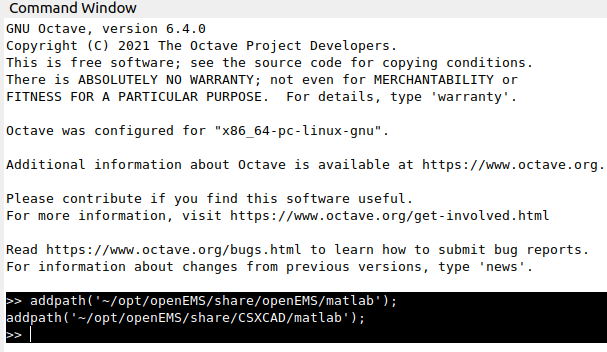
\includegraphics[width=\textwidth]{./img/octavepath.png}
	\caption{Configuración de \emph{path} en GNU Octave.}
	\label{fig:octavepath}
\end{figure}

El siguiente paso es verificar la interfaz CXCAD, a continuación se muestra el
comando y respuesta en la ventana de comandos de GNU Octave:

\begin{verbatim}
>> InitCSX
ans = 
Properties: []
\end{verbatim}

Con la interfaz inicializada se puede realizar una verificación de sus funciones
como se muestra a continuación:

\begin{verbatim}
>> InitFDTD('NrTS', 0, 'EndCriteria', 0)
ans = 
    ATTRIBUTE: [1x1 struct]
\end{verbatim}

El siguiente paso es verificar el correcto funcionamiento del simulador como se
muestra a continuación:

\begin{verbatim}
>> RunOpenEMS( '.', 'nonexistant.xml', '' )
[...]
Read openEMS xml file: nonexistant.xml ...
openEMS: Error File-Loading failed!!! File: nonexistant.xml
\end{verbatim}

El error que se muestra significa que el simulador funciona correctamente ya que
su argumento es un archivo inexistente. Sin embargo, el binario del simulador se
invocó sin problemas.

Es importante verificar que el programa de visualización de definiciones de
geometría funcione de forma correcta, esto se logra con el siguiente comando:

\begin{verbatim}
CSXGeomPlot('nonexistant.xml')
\end{verbatim}

La ventana de comandos debe arrojar un error ya que el archivo de geometría no
existe, sin embargo se debe ejecutar el visualizador como se muestra en la
figura \ref{fig:geovisual}.

Llegado a este punto se puede concluir que openEMS fue instalado de forma correcta.

\begin{figure}[htbp]
	\centering
	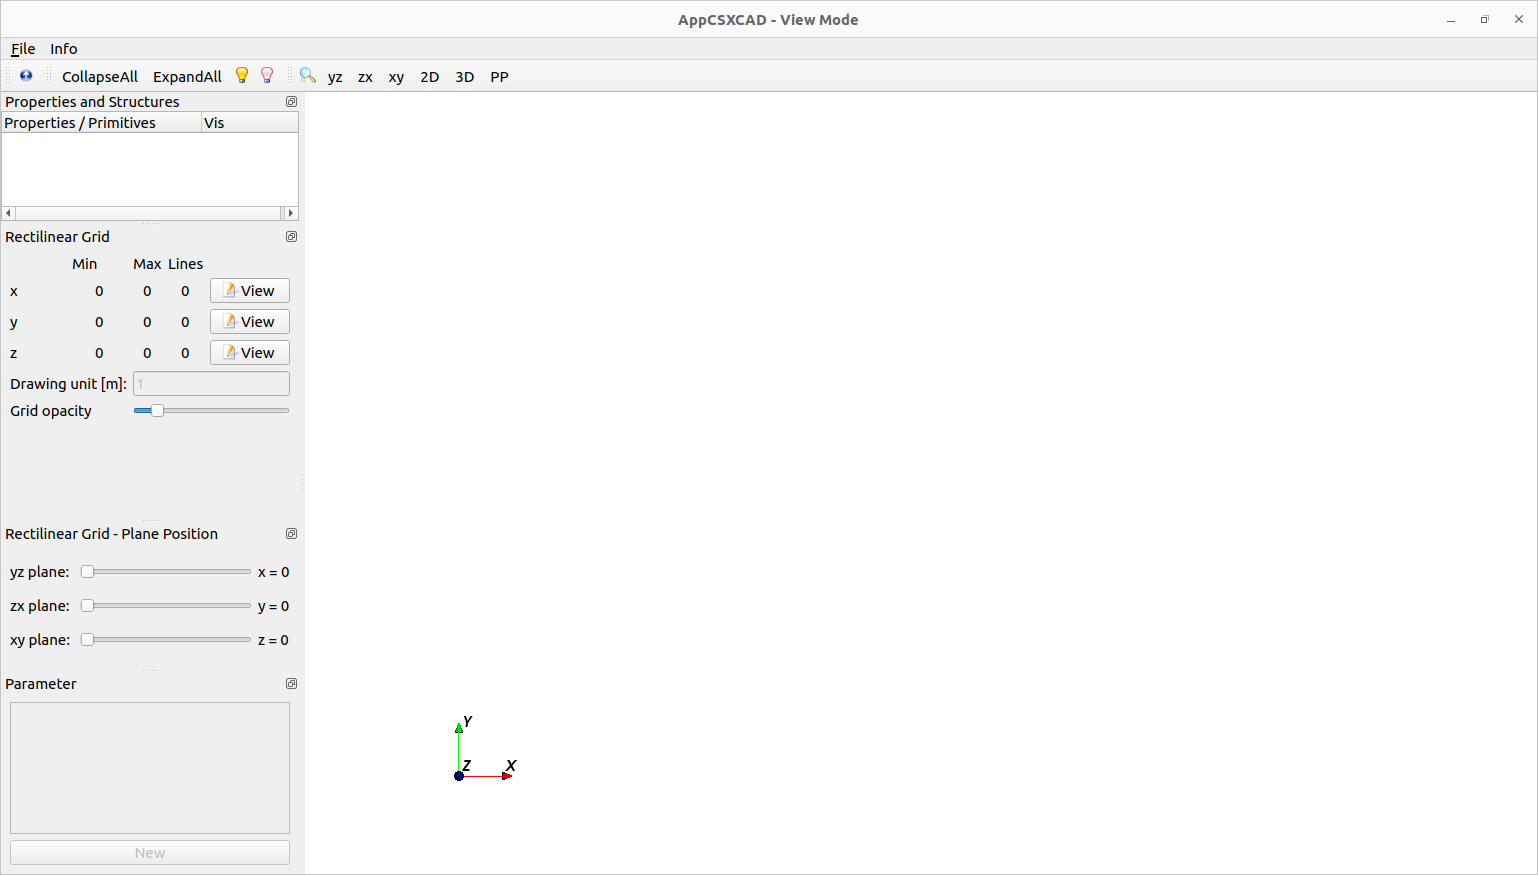
\includegraphics[width=\textwidth]{./img/geovisual.png}
	\caption{Programa de visualización de geometrías.}
	\label{fig:geovisual}
\end{figure}

Se recomienda instalar el programa ParaView para tener una herramienta para
visualizar las simulaciones.
Los ejemplos de este documento utilizan ParaView para representar de forma
gráfica los resultados.

\subsection{Ejemplos de uso}
\label{sub:oejemplos}

\subsubsection{Guía de onda superficial}
\label{subsub:oejemplo1}

Las instrucciones para generar la geometría, su excitación y la definición de
las variables a observar son las siguientes:

\begin{verbatim}
close all
clear
clc
FDTD = InitFDTD('NrTS',100, 'EndCriteria',0, 'OverSampling',50);
FDTD = SetSinusExcite(FDTD,10e6);
FDTD = SetBoundaryCond(FDTD,{'PMC' 'PMC' 'PEC' 'PEC' 'MUR' 'MUR'});
CSX = InitCSX();
mesh.x = -10:10;
mesh.y = -10:10;
mesh.z = -10:30;
CSX = DefineRectGrid(CSX, 1, mesh);
CSX = AddExcitation(CSX,'excitation',0,[0 1 0]);
CSX = AddBox(CSX,'excitation',0,[-10 -10 0],[10 10 0]);
CSX = AddDump(CSX,'Et');
CSX = AddBox(CSX,'Et',0,[-10 0 -10],[10 0 30]);
mkdir('tmp');
WriteOpenEMS('tmp/tmp.xml',FDTD,CSX);
\end{verbatim}

Antes de lanzar la simulación se procede a verificar la geometría generada con
los siguientes comandos:

\begin{verbatim}
CSXGeomPlot( 'tmp/tmp.xml' );
\end{verbatim}

En la figura \ref{fig:geo1} se puede observar el plano que simula una guía de onda.

\begin{figure}[htbp]
	\centering
	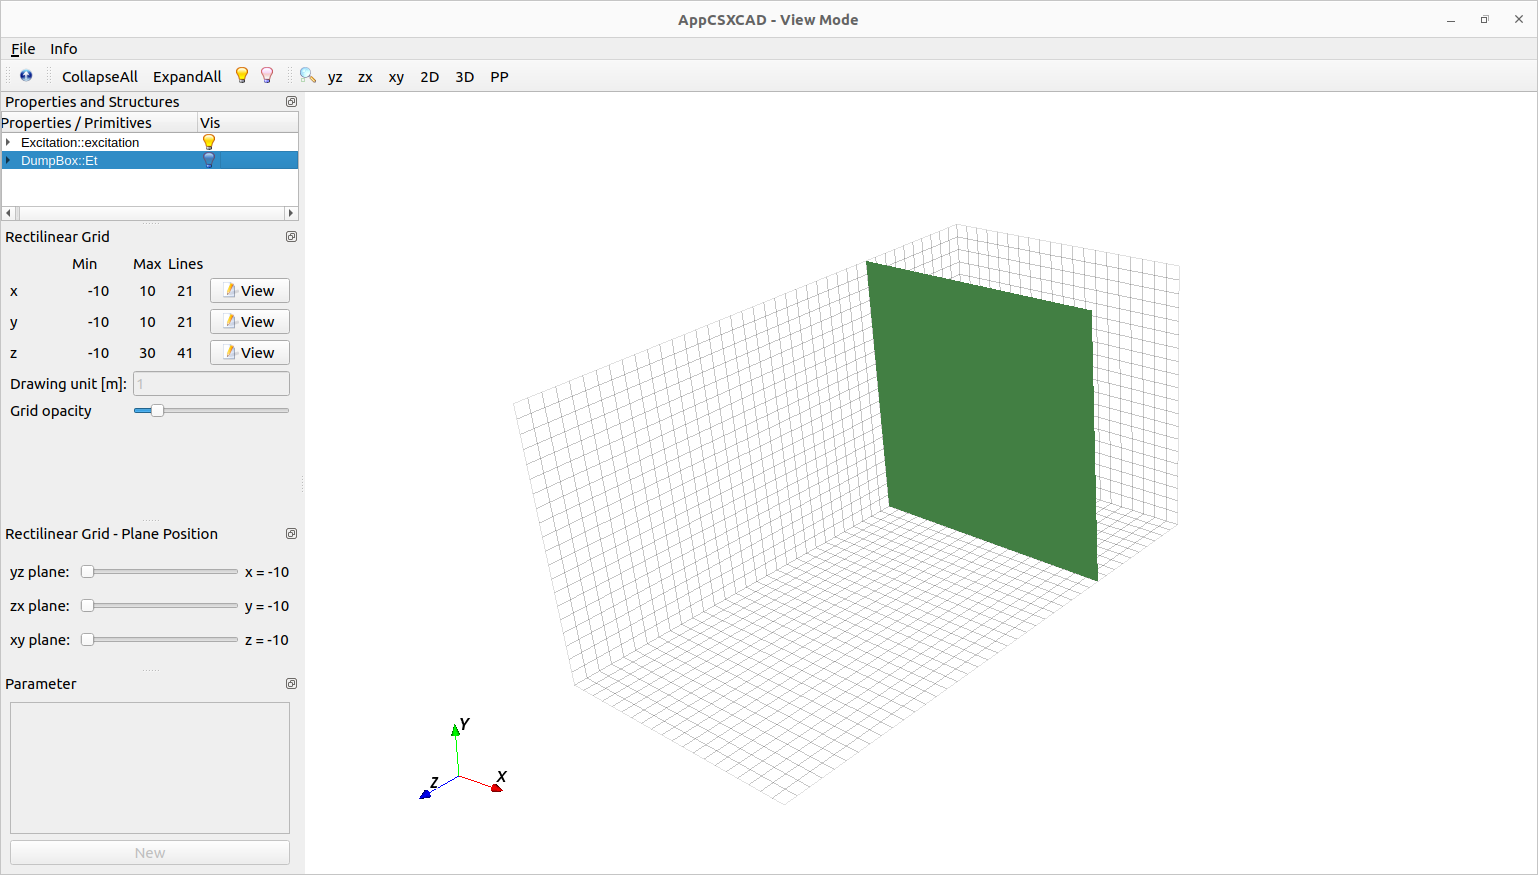
\includegraphics[width=\textwidth]{./img/geo1.png}
	\caption{Geometría del ejemplo 1.}
	\label{fig:geo1}
\end{figure}

Una vez satisfecho con la geometría, se procede a lanzar la simulación. Para
eso, primero debe cerrar el visualizador de geometría y escribir el siguiente
comando:

\begin{verbatim}
RunOpenEMS('tmp','tmp.xml','');
\end{verbatim}

Para visualizar la simulación se puede usar el programa ParaView. Para eso se
debe abrir el archivo \texttt{Et..vtr}, luego debe ingresar al inspector de
objetos y seleccionar que el color se asocie al \emph{E-Field} además de indicar
el eje \emph{Y}. Seguidamente,
puede hacer click en el boton de \emph{play}.
Se verá una animación con la variación del potencial eléctrico en el tiempo, sin
embargo los colores se encuentran sobre el plano y no se puede apreciar con
facilidad la onda.

Para mejorar la representación se debe colocar el filtro \emph{warp-by-vector}
que deformará la representación según la intensidad del campo, esto genera una
representación en donde se puede observar con facilidad la onda en la guía.

En la figura \ref{fig:sim1} se puede observar la guía de onda simulada en un plano.

\begin{figure}[htbp]
	\centering
	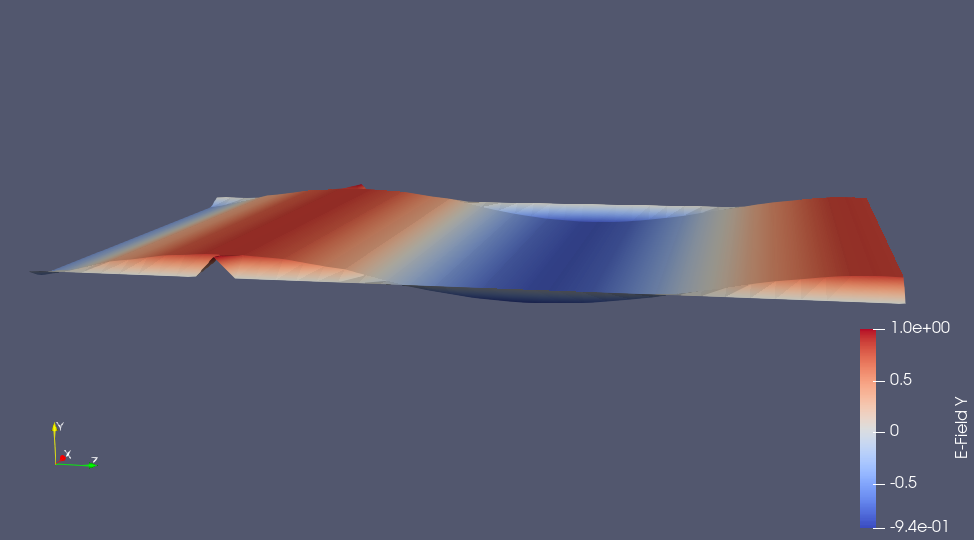
\includegraphics[width=\textwidth]{./img/sim1.png}
	\caption{Simulación del ejemplo 1.}
	\label{fig:sim1}
\end{figure}

\subsubsection{Esfera metálica dispersa un frente de onda}
\label{subsub:oejemplo2}

En este ejemplo se simula la dispersión que produce una esfera metálica cuando
una onda incide sobre ella.
Para tal fin se generó una geometría esférica con la propiedad física de ser un
conductor eléctrico. Se la puede ver en la figura \ref{fig:sim2}.

\begin{figure}[htbp]
	\centering
	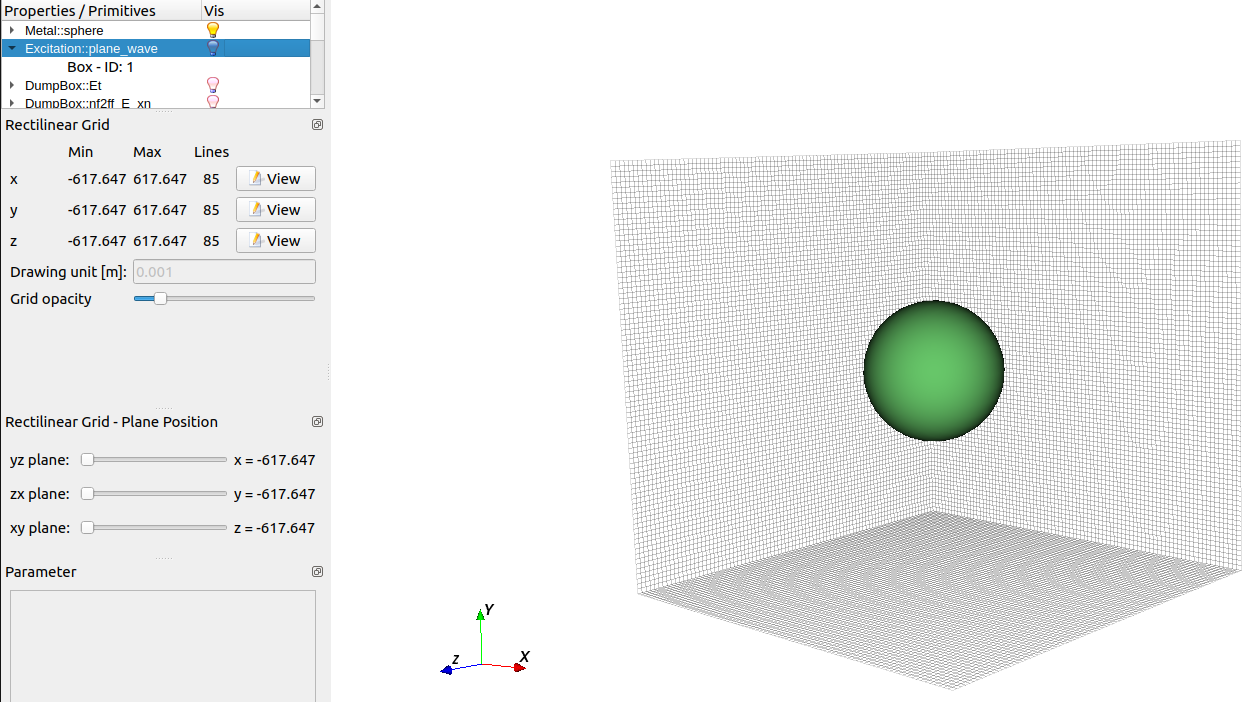
\includegraphics[width=\textwidth]{./img/ejemplo_esfera.png}
	\caption{Esfera metálica del ejemplo 2.}
	\label{fig:sim2}
\end{figure}

Luego se definió un cubo como volumen de simulación lo suficientemente grande
para que el cálculo numérico sea lo más preciso posible pero que los tiempos de
cómputo sean aceptables. El volumen se puede observar en la figura \ref{fig:sim3}.

\begin{figure}[htbp]
	\centering
	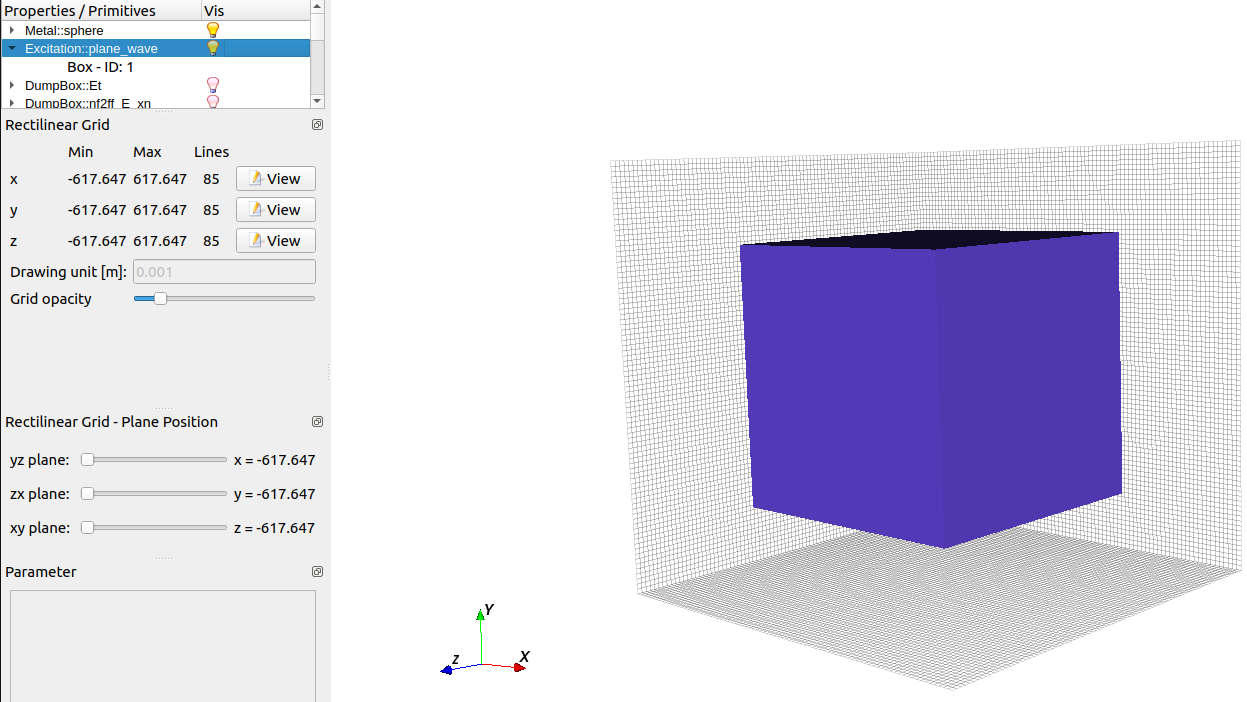
\includegraphics[width=\textwidth]{./img/ejemplo_cubo.png}
	\caption{Volumen de simulación del ejemplo 2.}
	\label{fig:sim3}
\end{figure}

Luego se corrió la simulación y se la visualizó con ParaView.
Se tomaron capturas en 3 momentos distintos y se los muestran en 2 y 3
dimensiones.
Se pueden observar en las figuras \ref{fig:sim4},\ref{fig:sim5},\ref{fig:sim6},\ref{fig:sim7},\ref{fig:sim8} y \ref{fig:sim9}.

A continuación se describe el código para generar el ejemplo:

\begin{verbatim}
% Si es la primera ejecución de octave de la sesión de trabajo
% agregar openEMS al path, sino physical_constants no va a estar
% definido
addpath('~/opt/openEMS/share/openEMS/matlab');
addpath('~/opt/openEMS/share/CSXCAD/matlab');

close all
clear
clc

%% Se configura la simulación
physical_constants;
unit = 1e-3; % longitudes en mm

sphere.rad = 200;

inc_angle = 0 /180*pi; % ángulo incidente (x-axis) en rad

% Tamaño de la caja de simulación
SimBox = 1000;
PW_Box = 750;

%% configuración FDTD parámetros y función de excitación
f_start =  50e6; % frecuencia de inicio
f_stop = 1000e6; % frecuencia de fin
f0 = 500e6;

FDTD = InitFDTD( );
FDTD = SetGaussExcite( FDTD, 0.5*(f_start+f_stop), 0.5*(f_stop-f_start) );
BC = [1 1 1 1 1 1]*3;  % set boundary conditions
FDTD = SetBoundaryCond( FDTD, BC );

%% configurar CSXCAD geometría y malla
max_res = c0 / f_stop / unit / 20; % cell size: lambda/20
CSX = InitCSX();

% creación de malla
smooth_mesh = SmoothMeshLines([0 SimBox/2], max_res);
mesh.x = unique([-smooth_mesh smooth_mesh]);
mesh.y = mesh.x;
mesh.z = mesh.x;

%% creación de esfera de metal
CSX = AddMetal( CSX, 'sphere' ); % se crea un conductor perfecto (PEC)
CSX = AddSphere(CSX,'sphere',10,[0 0 0],sphere.rad);

%% excitación de onda planar
k_dir = [cos(inc_angle) sin(inc_angle) 0]; % dirección de la onda planar
E_dir = [0 0 1]; % polarización de la onda planar --> E_z

CSX = AddPlaneWaveExcite(CSX, 'plane_wave', k_dir, E_dir, f0);
start = [-PW_Box/2 -PW_Box/2 -PW_Box/2];
stop  = -start;
CSX = AddBox(CSX, 'plane_wave', 0, start, stop);

CSX = AddDump(CSX, 'Et');
start = [mesh.x(1)   mesh.y(1)   0];
stop  = [mesh.x(end) mesh.y(end) 0];
CSX = AddBox(CSX, 'Et', 0, start, stop);

%% cálculo nf2ff
start = [mesh.x(1)     mesh.y(1)     mesh.z(1)];
stop  = [mesh.x(end) mesh.y(end) mesh.z(end)];
[CSX nf2ff] = CreateNF2FFBox(CSX, 'nf2ff', start, stop);

mesh = AddPML(mesh,8);

CSX = DefineRectGrid( CSX, unit, mesh );

%% carpeta de simulación
Sim_Path = 'Sphere_RCS';
Sim_CSX = 'Sphere_RCS.xml';

[status, message, messageid] = rmdir( Sim_Path, 's' );
[status, message, messageid] = mkdir( Sim_Path );

WriteOpenEMS( [Sim_Path '/' Sim_CSX], FDTD, CSX );

%% Se muestra la geometría
CSXGeomPlot( [Sim_Path '/' Sim_CSX] );

%% se corre la simulación
RunOpenEMS( Sim_Path, Sim_CSX);
\end{verbatim}
\begin{figure}[htbp]
	\centering
	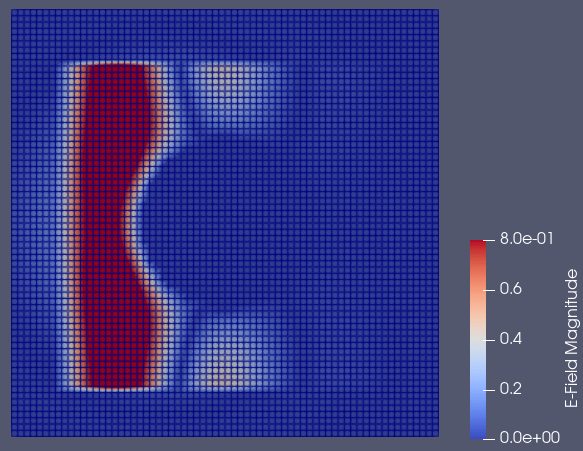
\includegraphics[width=\textwidth]{./img/impacto.png}
	\caption{Simulación momento 1.}
	\label{fig:sim4}
\end{figure}

\begin{figure}[htbp]
	\centering
	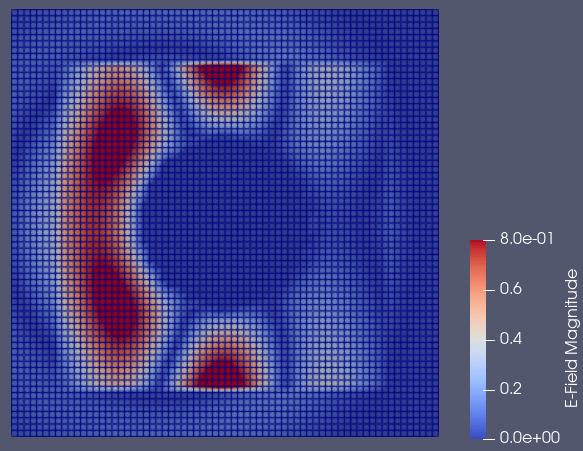
\includegraphics[width=\textwidth]{./img/mitad.png}
	\caption{Simulación momento 2.}
	\label{fig:sim5}
\end{figure}

\begin{figure}[htbp]
	\centering
	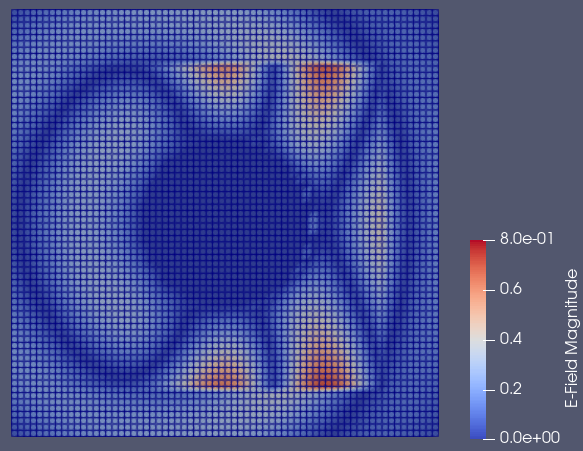
\includegraphics[width=\textwidth]{./img/salida.png}
	\caption{Simulación momento 3.}
	\label{fig:sim6}
\end{figure}

\begin{figure}[htbp]
	\centering
	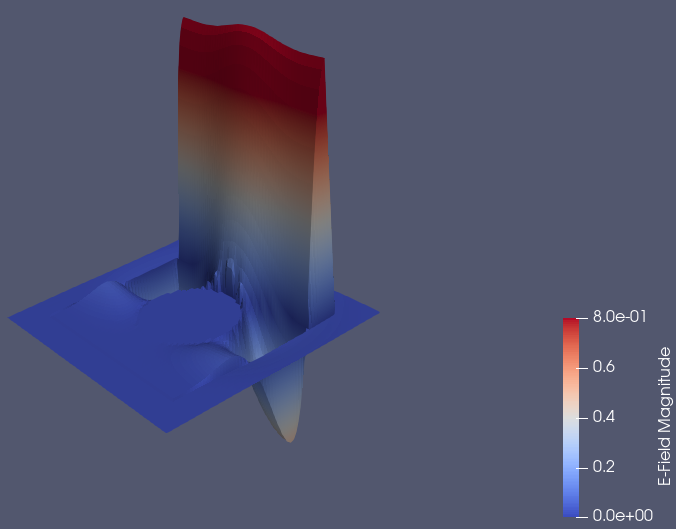
\includegraphics[width=\textwidth]{./img/impacto3d.png}
	\caption{Simulación momento 1 en 3D.}
	\label{fig:sim7}
\end{figure}

\begin{figure}[htbp]
	\centering
	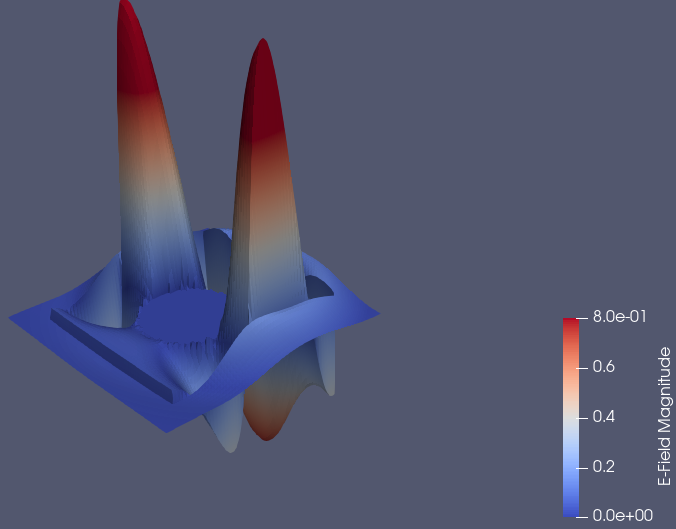
\includegraphics[width=\textwidth]{./img/mitad3d.png}
	\caption{Simulación momento 2 en 3D.}
	\label{fig:sim8}
\end{figure}

\begin{figure}[htbp]
	\centering
	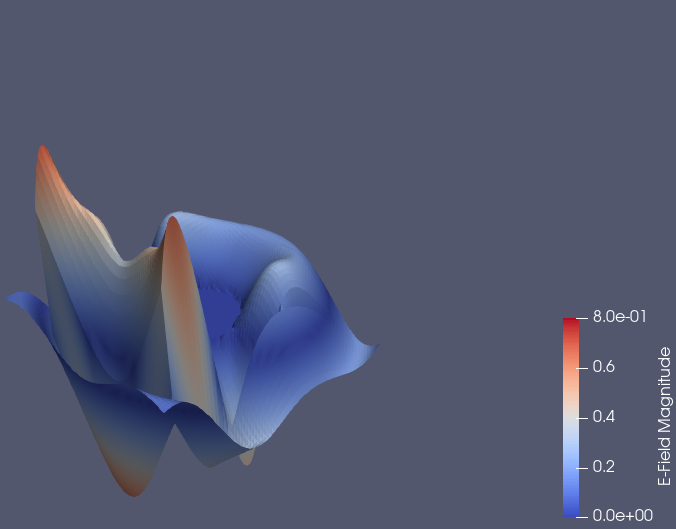
\includegraphics[width=\textwidth]{./img/salida3d.png}
	\caption{Simulación momento 3 en 3D.}
	\label{fig:sim9}
\end{figure}

\subsection{Primeros intentos de simular circuitos impresos}

OpenEMS utiliza un \emph{parser} para transformar los archivos \emph{HyperLynx}
que exportan programas como KiCad e Eagle en un formato que el motor de matlab pueda entender.
Sin embargo, el \emph{parser} hyp2mat es un programa cuyo único autor dió por finalizado y quedaron deprecadas las
recetas de Autotools y las bibliotecas que utiliza para \emph{linkear}.

Existen tres posibilidades en este punto:

\begin{itemize}
	\item Crear un dockerfile que genere una imagen con Octave y OpenEMS en base a una versión de Ubuntu 
	que soporte la última versión de hyp2mat que se publicó.
	\item Utilizar un método alternativo para importar los circuitos impresos.
	\item Abandonar OpenEMS como herramienta viable.
\end{itemize}

\subsection{Montaje de GNU/Octave y OpenEMS en docker}

Se pudo crear una serie de recetas que generan una imagen y contenedor con Octave y OpenEMS.

Dockerfile:

\begin{verbatim}
# Universidad Nacional de la Matanza.

# Los Dockerfiles comienzan a partir de una imagen base
FROM ubuntu:focal

# En esta sección se actualiza la base de datos del gestor
# de paquetes (apt) y se procede a instalar las herramientas
# y sus dependencias
RUN apt-get update &&  DEBIAN_FRONTEND=noninteractive apt-get install -y -q \
  octave-common \
  openems \
  octave-openems \
  libcsxcad0

# Se genera un usuario de desarrollo (dev) con permisos de
# administrador y sin necesidad de ingresar su contraseña
RUN adduser --disabled-password --gecos '' dev && \
  usermod -aG sudo dev && \
  echo "dev ALL=(ALL) NOPASSWD: ALL" >> /etc/sudoers

# Se hace /bin/sh symlink a bash en vez de dash:
RUN echo "dash dash/sh boolean false" | debconf-set-selections
RUN DEBIAN_FRONTEND=noninteractive dpkg-reconfigure dash

# Cuando se ingrese al contenedor se ingresara como dev
USER dev
ENV HOME /home/dev
ENV LANG en_US.UTF-8

# Se crea una carpeta de trabajo y se la configura como
# workdir
RUN mkdir /home/dev/workspace
WORKDIR /home/dev/workspace
\end{verbatim}

Receta de creación:

\begin{verbatim}
#!/bin/bash
docker build \
    -t openems .
\end{verbatim}

Receta de lanzamiento del contenedor:

\begin{verbatim}
#!/bin/bash

# El comentario que comienza con un signo de exclamacion
# tiene la finalidad de indicarle al sistema con que binario
# debe ejecutar este archivo, en nuestro caso el intérprete de
# BASH

# Se define el directorio del host como "path to working directory"
# (PWD), esto es, la carpeta desde donde lanzamos este script.
DIRECTORIO_DE_MI_MAQUINA=PWD

docker run -ti \
    -e DISPLAY=$DISPLAY \
    --net="host" \
    --name="UNLaM" \
    --hostname="UNLAM" \
    -v $DIRECTORIO_DE_MI_MAQUINA:/home/dev/workspace \
    openems
    /bin/bash
\end{verbatim}

\begin{figure}[htbp]
	\centering
	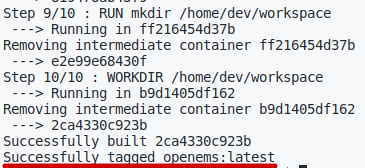
\includegraphics[width=0.5\textwidth]{./img/docker-build.png}
	\caption{Construcción de imagen}
	\label{fig:dockerbuild}
\end{figure}

\begin{figure}[htbp]
	\centering
	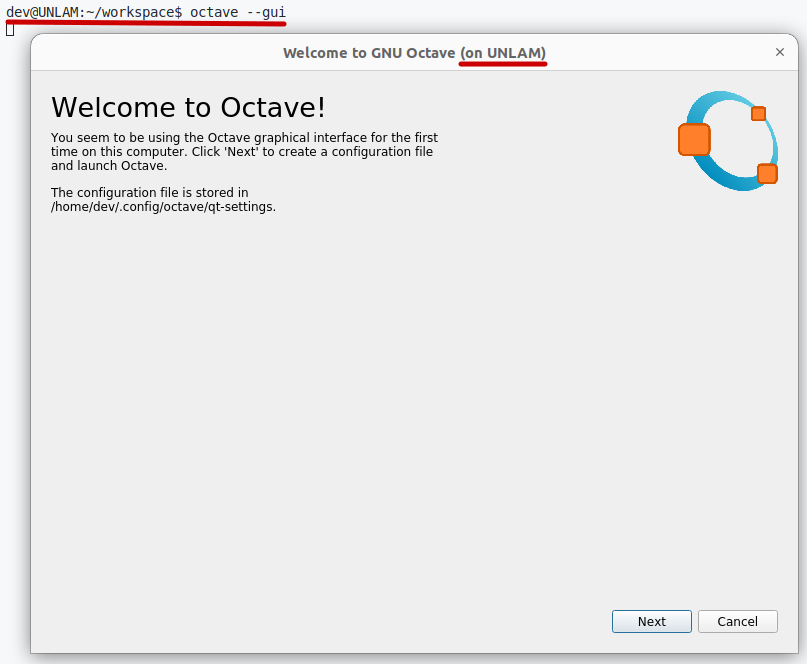
\includegraphics[width=\textwidth]{./img/docker-run.png}
	\caption{Ejecución del contenedor}
	\label{fig:dockerrun}
\end{figure}

\newpage

%%%%%%%%%%%%%%%%%%%%%%%%%%%%%%%%%%%%%%%%%%%%%%%%%%%%%%%%%%%%%%%%%%%%%%%%%%%%%%%

\section{Ansys}

Ansys HFSS (simulador de estructura de alta frecuencia) es un solucionador comercial de métodos de elementos finitos para estructuras electromagnéticas (EM) de Ansys que ofrece varias tecnologías de resolución de última generación.
Cada solucionador en ANSYS HFSS es un procesador de solución automatizado para el cual el usuario dicta la geometría, las propiedades del material y el rango requerido de frecuencias de solución.

Los ingenieros utilizan Ansys HFSS principalmente para diseñar y simular componentes electrónicos de alta velocidad y alta frecuencia en sistemas de radar, sistemas de comunicación, satélites, ADAS, microchips, placas de circuito impreso, productos IoT y otros dispositivos digitales y dispositivos RF.
El solucionador también se ha utilizado para simular el comportamiento electromagnético de objetos como automóviles y aviones.
ANSYS HFSS permite a los diseñadores de sistemas y circuitos simular problemas de EM, como pérdidas por atenuación, acoplamiento, radiación y reflexión.

HFSS captura y simula objetos en 3D, teniendo en cuenta la composición de los materiales y las formas/geometrías de cada objeto.
Además, está preparada para ser utilizadas en el diseño de antenas y elementos complejos de circuitos electrónicos de radiofrecuencia, incluidos filtros, líneas de transmisión y empaques.

Durante el transcurso del 2022 se logró un contacto comercial que realizó una propuesta de trabajo a la UNLaM a cambio de licencias y capacitación.
Se dió una capacitación sobre la funcionalidad y sinergia entre los distintos motores de físicas.

\begin{figure}[htbp]
	\centering
	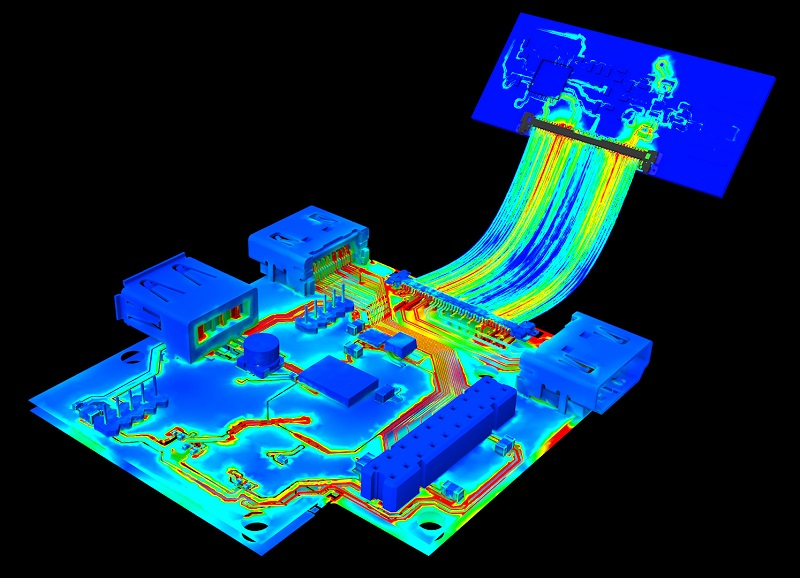
\includegraphics[width=0.8\textwidth]{img/ansys.jpg}
	\caption{Simulación de PCB flexible en Ansys.}
	\label{fig:ansys}
\end{figure}

\newpage

%%%%%%%%%%%%%%%%%%%%%%%%%%%%%%%%%%%%%%%%%%%%%%%%%%%%%%%%%%%%%%%%%%%%%%%%%%%%%%%

\section{Elmer}

Elmer es un software de simulación multi-física de código abierto desarrollado principalmente por \emph{IT Center for Science} (CSC).
El desarrollo de Elmer se inició como una colaboración nacional con las universidades finlandesas, los institutos de investigación y la industria.

Elmer incluye modelos físicos de dinámica de fluidos, mecánica estructural, electromagnetismo, transferencia de calor y acústica.
Estos se describen mediante ecuaciones diferenciales parciales que Elmer resuelve mediante el método de elementos finitos (FEM).
Elmer admite computación paralela.

Actualmente los campos de uso más destacados son la glaciología computacional y el electromagnetismo computacional.

\begin{figure}[htbp]
	\centering
	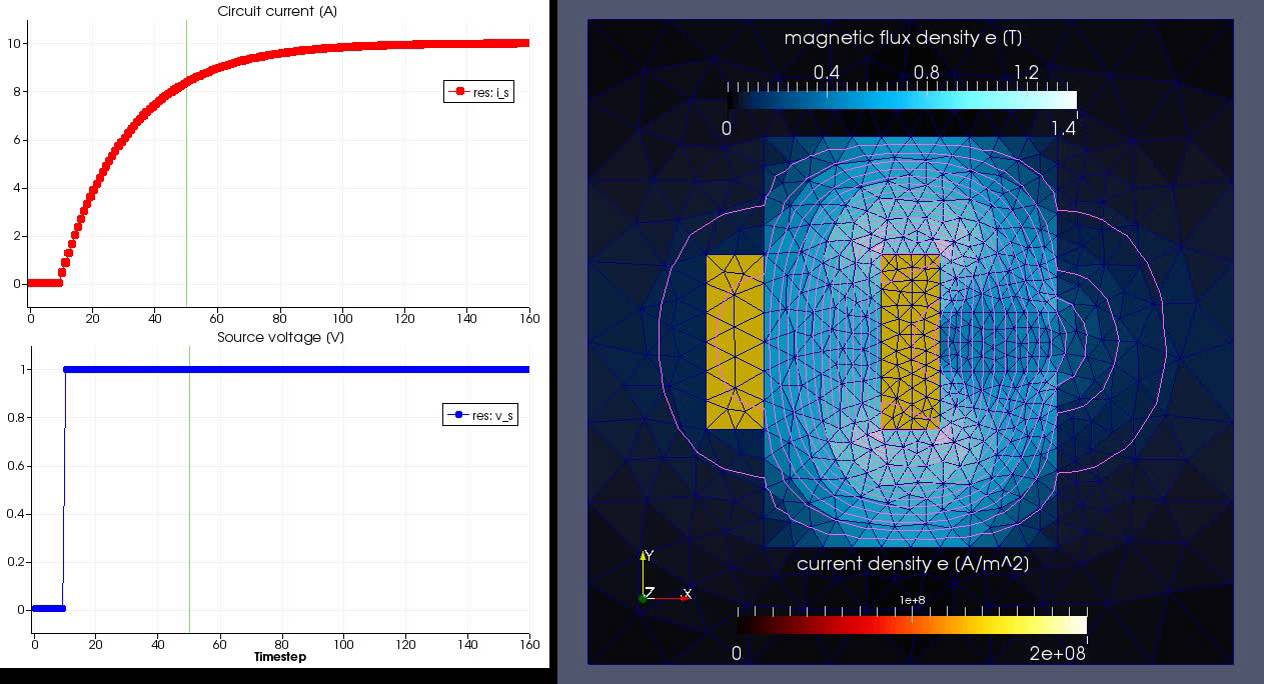
\includegraphics[width=0.8\textwidth]{img/elmer.jpg}
	\caption{Simulación en Elmer.}
	\label{fig:elmer}
\end{figure}

\newpage

\section{Conclusiones}

\begin{itemize}
	\item OpenEMS: el programa no logró cumplir las expectativas y no se ajusta a las necesidades académicas. No se recomienda para su uso ni continuar su investigación.
	\item Ansys: a pesar que el programa es propietario y demandaría un costo económico para la universidad, se ajusta a las necesidades académicas. Se recomienda continuar con su investigación.
	\item Elmer: se debe comenzar su investigación. Esto significa comenzar con sus pruebas de simulación y flujo de trabajo.
\end{itemize}

\end{document}
